\chapter{Архитектура Faster R-CNN} \label{appendix1}							% 
%\addcontentsline{toc}{chapter}{Архитектура Faster R-CNN}	% Добавляем его в оглавление

Полная архитектура Faster R-CNN выглядит следующим образом:

\begin{figure}
%	\center
	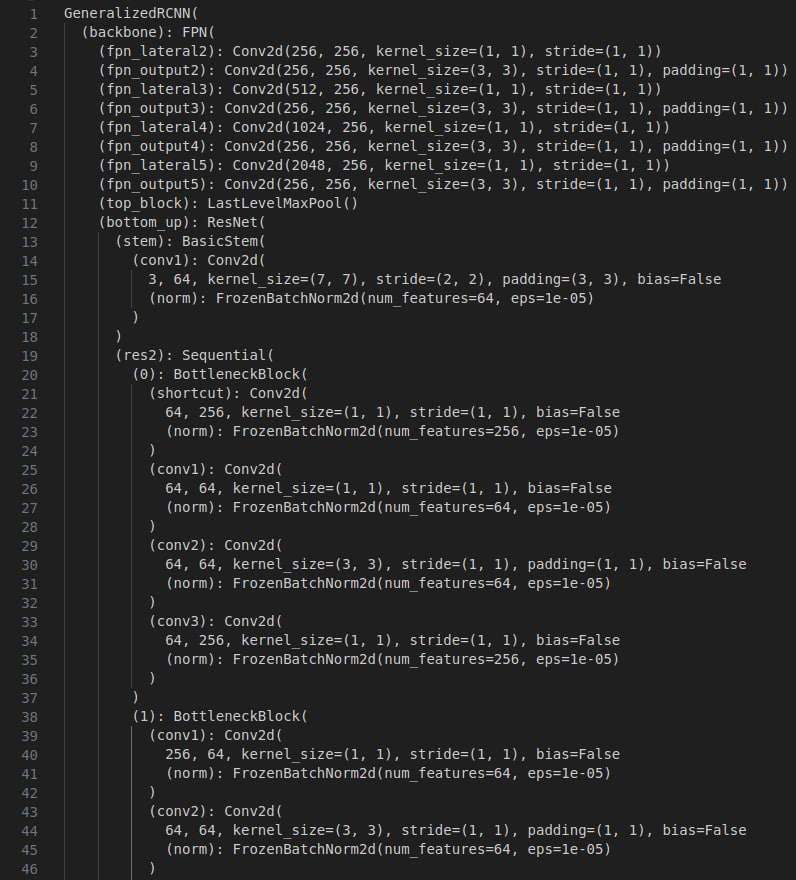
\includegraphics [scale=0.3]{my_folder/images/arch1}
	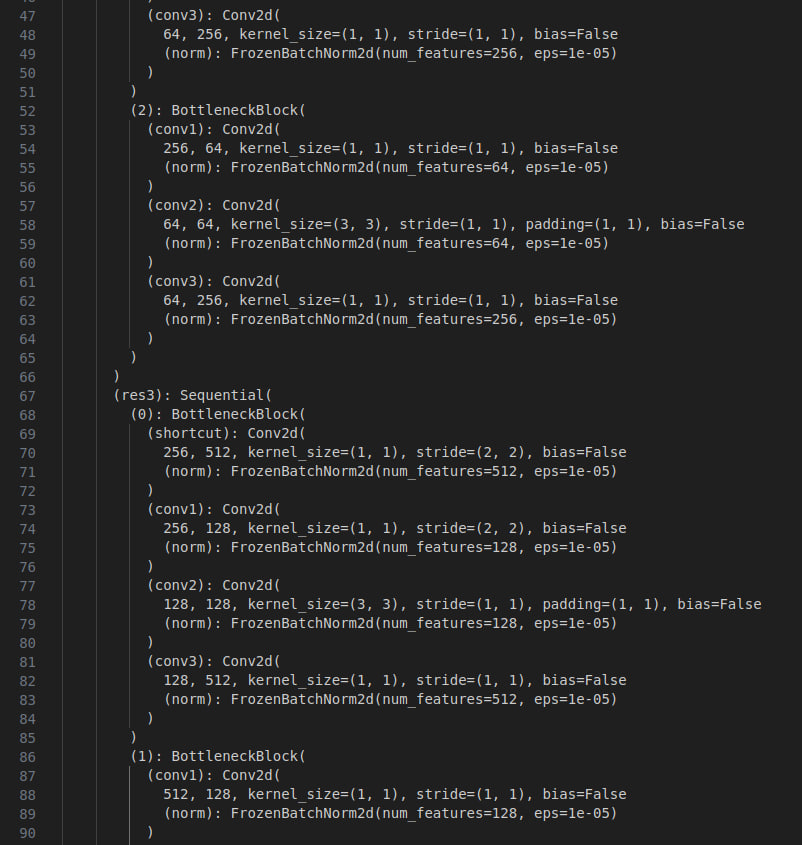
\includegraphics [scale=0.3]{my_folder/images/arch2}
	\label{fig:arch12}
	\caption{Архитектура Faster R-CNN (1)}
\end{figure}
\begin{figure}
%	\center
	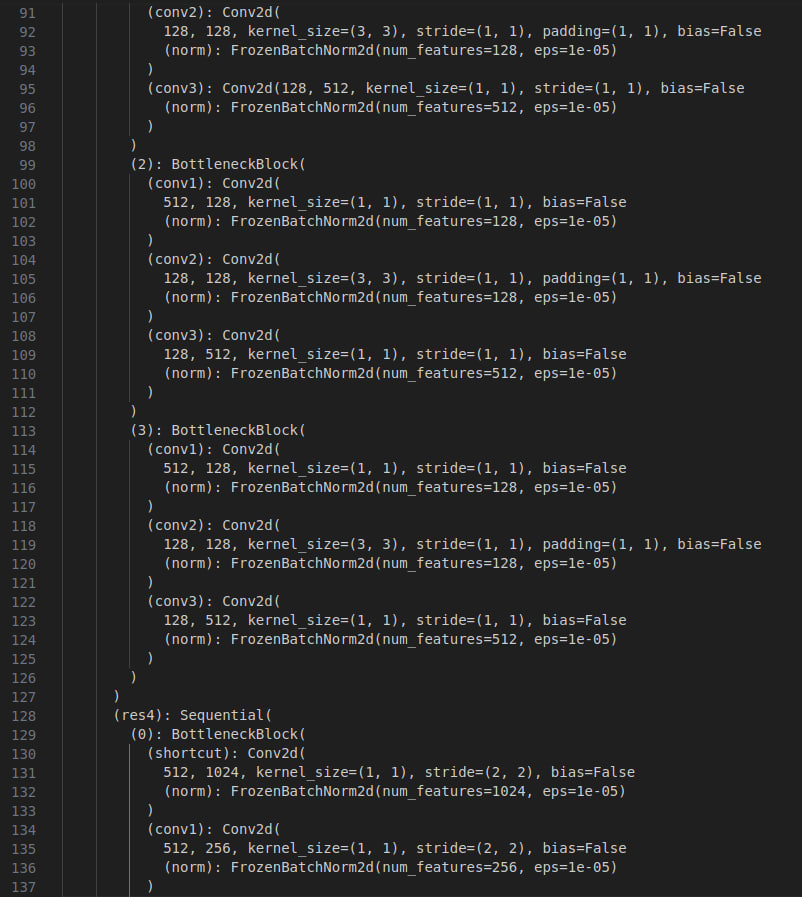
\includegraphics [scale=0.3]{my_folder/images/arch3}
	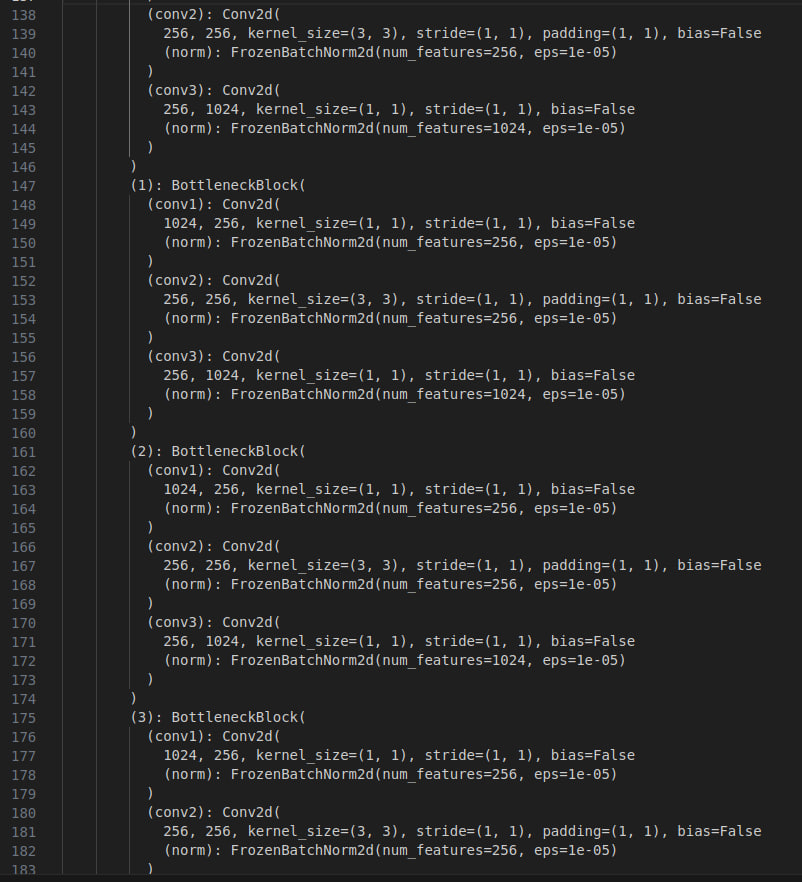
\includegraphics [scale=0.3]{my_folder/images/arch4}
	\label{fig:arch34}
	\caption{Архитектура Faster R-CNN (2)}
\end{figure}
\begin{figure}
%	\center
	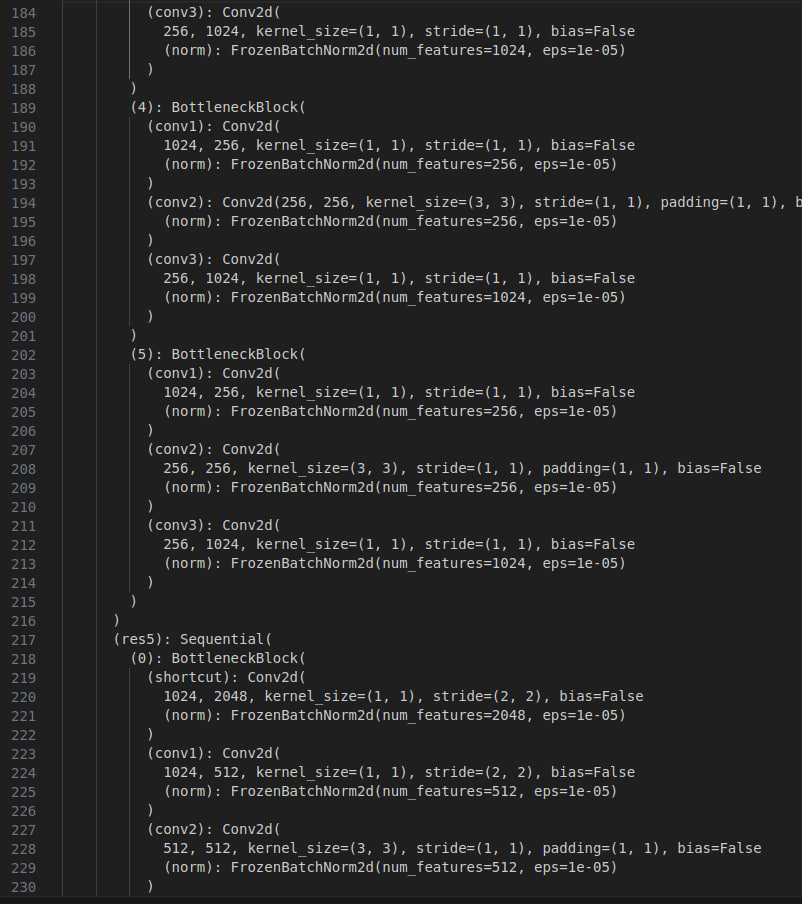
\includegraphics [scale=0.3]{my_folder/images/arch5}
	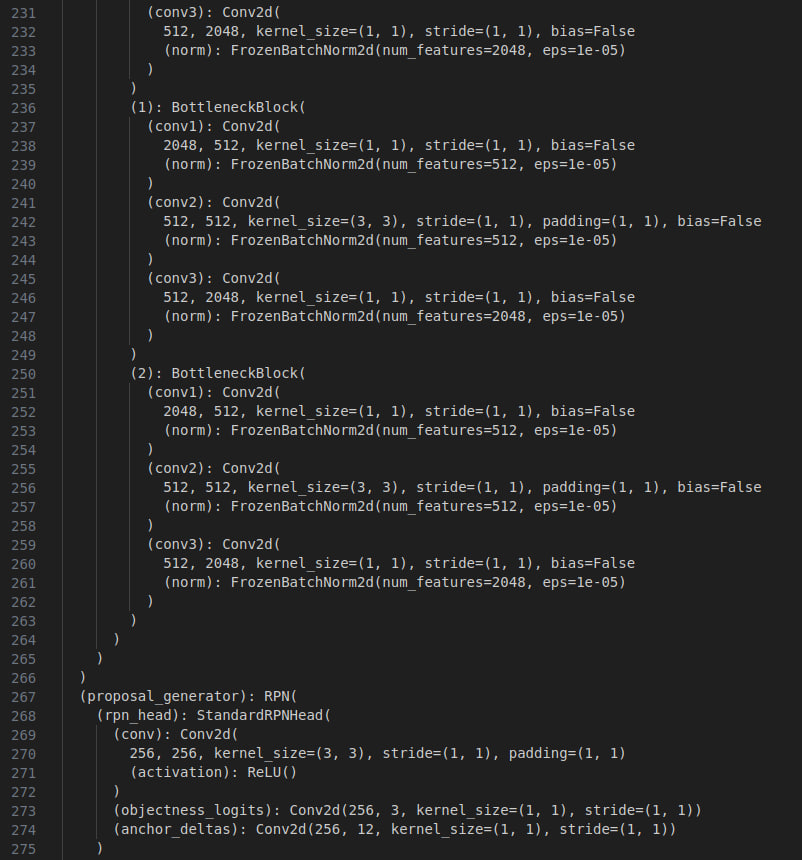
\includegraphics [scale=0.3]{my_folder/images/arch6}
	\label{fig:arch56}
	\caption{Архитектура Faster R-CNN (3)}
\end{figure}
\begin{figure}
%	\center
	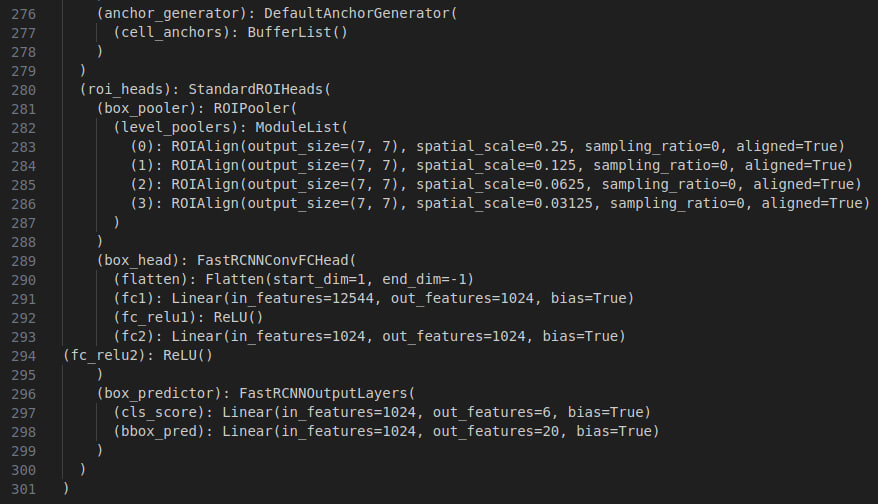
\includegraphics [scale=0.6]{my_folder/images/arch7}
	\caption{Архитектура Faster R-CNN (4)}
	\label{fig:arch7}
\end{figure}
%
%% В случае, когда таблица (рисунок) размещаются на последней странице, для переноса названия приложения на новую строку используем:
%\NewPage % начать новое приложение с новой страницы 